%-----------------------------------------------------------------------
%
%     This file is part of the Code_Saturne Kernel, element of the
%     Code_Saturne CFD tool.
%
%     Copyright (C) 1998-2008 EDF S.A., France
%
%     contact: saturne-support@edf.fr
%
%     The Code_Saturne Kernel is free software; you can redistribute it
%     and/or modify it under the terms of the GNU General Public License
%     as published by the Free Software Foundation; either version 2 of
%     the License, or (at your option) any later version.
%
%     The Code_Saturne Kernel is distributed in the hope that it will be
%     useful, but WITHOUT ANY WARRANTY; without even the implied warranty
%     of MERCHANTABILITY or FITNESS FOR A PARTICULAR PURPOSE.  See the
%     GNU General Public License for more details.
%
%     You should have received a copy of the GNU General Public License
%     along with the Code_Saturne Kernel; if not, write to the
%     Free Software Foundation, Inc.,
%     51 Franklin St, Fifth Floor,
%     Boston, MA  02110-1301  USA
%
%-----------------------------------------------------------------------
%


\programme{cfxtcl}
%
\vspace{1cm}
%%%%%%%%%%%%%%%%%%%%%%%%%%%%%%%%%%
%%%%%%%%%%%%%%%%%%%%%%%%%%%%%%%%%%
\section{Fonction}
%%%%%%%%%%%%%%%%%%%%%%%%%%%%%%%%%%
%%%%%%%%%%%%%%%%%%%%%%%%%%%%%%%%%%

Pour le traitement des conditions aux limites, on consid\`ere
le syst\`eme (\ref{Cfbl_Cfxtcl_eq_ref_laminaire_cfxtcl})

\begin{equation}\label{Cfbl_Cfxtcl_eq_ref_laminaire_cfxtcl}
\left\{\begin{array}{l}

\displaystyle\frac{\partial\rho}{\partial t} + \divs(\vect{Q}) = 0 \\
\\
\displaystyle\frac{\partial\vect{Q}}{\partial t}
+ \divv(\vect{u} \otimes \vect{Q}) + \gradv{P}
= \rho \vect{f}_v + \divv(\tens{\Sigma}^v) \\
\\
\displaystyle\frac{\partial E}{\partial t} + \divs( \vect{u} (E+P) )
= \rho\vect{f}_v\cdot\vect{u} + \divs(\tens{\Sigma}^v \vect{u})
- \divs{\,\vect{\Phi}_s} + \rho\Phi_v

\end{array}\right.
\end{equation}

en tant que syst\`eme hyperbolique portant sur la variable vectorielle
$\vect{W}=\ ^t(\rho,\vect{Q},E)$.

Le syst\`eme s'\'ecrit alors~:
\begin{equation}\label{Cfbl_Cfxtcl_eq_hyperbolique_cfxtcl}
\displaystyle\frac{\partial \vect{W}}{\partial t}
+ \displaystyle\sum\limits_{i=1}^3
\frac{\partial}{\partial x_i}\vect{F}_i(\vect{W})
= \displaystyle\sum\limits_{i=1}^3
\frac{\partial}{\partial x_i}\vect{F}_i^D(\vect{W},\nabla \vect{W})
+ \vect{\mathcal{S}}
\end{equation}
o\`u les $\vect{F}_i(\vect{W})$ sont les vecteurs flux convectifs
et les $\vect{F}_i^D(\vect{W})$ sont les vecteurs flux diffusifs
dans les trois directions d'espace,
et $\vect{\mathcal{S}}$ est un terme source.

La d\'emarche classique de \CS est adopt\'ee~: on impose les conditions
aux limites en d\'eterminant, pour chaque variable, des valeurs num\'eriques
de bord. Ces valeurs sont calcul\'ees de telle fa\c con que, lorsqu'on
les utilise dans les formules standard donnant les flux discrets, on obtienne
les contributions souhait\'ees au bord.

Pour rendre compte des flux convectifs (aux entr\'ees et aux sorties en particulier),
on fait abstraction des flux diffusifs et des termes
sources pour r\'esoudre un probl\`eme de Riemann qui
fournit un vecteur d'\'etat au bord. Celui-ci permet de calculer un flux,
soit directement (par les formules discr\`etes standard),
soit en appliquant un sch\'ema de Rusanov (sch\'ema de flux d\'ecentr\'e).

En paroi, on r\'esout  \'egalement, dans certains cas, un probl\`eme de
Riemann pour d\'eterminer une pression au bord.

%%%%%%%%%%%%%%%%%%%%%%%%%%%%%%%%%%
%%%%%%%%%%%%%%%%%%%%%%%%%%%%%%%%%%
\section{Discr\'etisation}
%%%%%%%%%%%%%%%%%%%%%%%%%%%%%%%%%%
%%%%%%%%%%%%%%%%%%%%%%%%%%%%%%%%%%

%=================================
\subsection{Introduction}
%=================================

%---------------------------------
\subsubsection{Objectif}
%---------------------------------

On r\'esume ici les diff\'erentes conditions aux limites utilis\'ees pour l'algorithme
compressible afin de fournir une vue d'ensemble. Pour atteindre cet objectif,
il est n\'ecessaire de faire r\'ef\'erence \`a  des \'el\'ements relatifs
\`a la discr\'etisation et au mode d'implantation des conditions aux limites.

Lors de l'implantation, on a cherch\'e \`a pr\'eserver la coh\'erence avec l'approche
utilis\'ee dans le cadre standard de l'algorithme incompressible de \CS.
Il est donc conseill\'e d'avoir pris connaissance du mode de traitement des conditions
aux limites incompressibles avant d'aborder les d\'etails de l'algorithme compressible.

Comme pour l'algorithme incompressible, les conditions aux limites sont impos\'ees
par le biais d'une valeur de bord associ\'ee \`a chaque variable. De plus,
pour certaines
fronti\`eres (parois \`a temp\'erature impos\'ee ou \`a flux thermique impos\'e),
on dispose de deux valeurs de bord pour la m\^eme variable, l'une d'elles \'etant d\'edi\'ee au calcul du
flux diffusif.
Enfin, sur certains types d'entr\'ee et de sortie, on d\'efinit \'egalement
une valeur du flux convectif au bord.

Comme pour l'algorithme incompressible, l'utilisateur peut d\'efinir,
pour chaque face
de bord, des conditions aux limites pour chaque variable, mais on conseille cependant
d'utiliser uniquement les types pr\'ed\'efinis
d\'ecrits ci-apr\`es (entr\'ee,
sortie, paroi, sym\'etrie) qui ont l'avantage d'assurer la coh\'erence entre
les diff\'erentes variables et les diff\'erentes \'etapes de calcul.


%---------------------------------
\subsubsection{Parois}
%---------------------------------

{\bf Pression} : on doit disposer d'une condition pour le calcul du gradient
qui intervient dans l'\'etape de quantit\'e de mouvement.
On dispose de deux types de condition, au choix de l'utilisateur~:
\begin{itemize}
\item par d\'efaut, la pression impos\'ee au bord est proportionnelle
\`a la valeur interne (la pression au bord est obtenue comme solution
d'un probl\`eme de Riemann sur les \'equations d'Euler
avec un \'etat miroir~; on distingue les cas de choc et de
d\'etente et, dans le cas d'une d\'etente trop forte, une condition de
Dirichlet homog\`ene est utilis\'ee pour \'eviter de voir appara\^itre une
pression n\'egative),
\item si l'utilisateur le souhaite (\var{ICFGRP(IPHAS)=1}), le gradient de
pression est impos\'e \`a partir du profil de pression hydrostatique.
\end{itemize}
\bigskip

{\bf Vitesse et turbulence}~: traitement standard (voir la documentation des
sous-programmes \fort{condli}
et \fort{clptur}).

{\bf Scalaires passifs}~: traitement standard
(flux nul par d\'efaut impos\'e dans \fort{typecl}).

{\bf Masse volumique}~: traitement standard des scalaires
(flux nul par d\'efaut impos\'e dans \fort{typecl}).

{\bf \'Energie et temp\'erature\footnote{Le gradient de temp\'erature est
{\it a priori} inutile, mais peut \^etre requis par l'utilisateur.}}~:
traitement standard des scalaires
(flux nul par d\'efaut impos\'e dans \fort{typecl}), hormis pour le
calcul du flux diffusif dans le cas de parois \`a temp\'erature impos\'ee
ou \`a flux thermique impos\'e.

{\bf Flux diffusif pour l'\'energie en paroi}~:
l'utilisateur peut choisir (dans \fort{uscfcl}) entre une temp\'erature de paroi impos\'ee
et un flux thermique diffusif (ou "conductif") impos\'e.
S'il ne pr\'ecise rien, on consid\`ere que la paroi est adiabatique
(flux thermique diffusif impos\'e et de valeur nulle).
Dans tous les cas, il faut donc disposer d'un moyen d'imposer le flux diffusif
souhait\'e. Pour cela, on d\'etermine une valeur de bord pour l'\'energie
qui, introduite dans la formule donnant le flux discret, permettra
d'obtenir la contribution attendue
(voir le paragraphe~\ref{Cfbl_Cfxtcl_section_cl_flux_diffusif_energie_cfener}).
Conform\'ement \`a l'approche classique de \CS, cette valeur est
stock\'ee sous la forme d'un couple de coefficients
(de type \var{COEFAF}, \var{COEFBF}).
Il est important de souligner que cette valeur de bord
ne doit \^etre utilis\'ee que pour le calcul
du flux diffusif~: dans les autres situations pour lesquelles
une valeur de bord de l'\'energie ou de la temp\'erature est requise
(calcul de gradient par exemple), on utilise une condition de flux nul
(traitement standard des scalaires). Pour cela, on dispose d'une
seconde valeur de bord qui est stock\'ee au moyen d'un
couple de coefficients (\var{COEFA}, \var{COEFB}) distinct du pr\'ec\'edent.
        
{\bf Flux convectifs}~: le flux de masse dans la direction normale \`a la paroi est
pris nul. De ce fait, les flux convectifs seront nuls quelle que soit les valeurs
de bord impos\'ees pour les diff\'erentes variables transport\'ees.

%---------------------------------
\subsubsection{Sym\'etrie}
%---------------------------------

Les conditions appliqu\'ees sont les conditions classiques de l'algorithme
incompressible (vitesse normale nulle, flux nul pour les autres variables).

Elles sont impos\'ees dans le sous-programme \fort{typecl} essentiellement. Pour
la pression, la condition de flux nul est impos\'ee dans \fort{cfxtcl}
(au d\'ebut des d\'eveloppements, on appliquait le m\^eme traitement qu'en paroi,
mais une condition de flux nul a \'et\'e pr\'ef\'er\'ee afin de s'affranchir des
probl\`emes potentiels dans les configurations 2D).


%---------------------------------
\subsubsection{Entr\'ees et sorties}
%---------------------------------

On obtient, par r\'esolution d'un probl\`eme de Riemann au bord, compl\'et\'e par
des relations de thermodynamique (\fort{uscfth}), des valeurs de bord pour toutes
les variables (on suppose qu'en entr\'ee, toutes les composantes de la vitesse
sont fournies~; elles sont suppos\'ees nulles par d\'efaut, hormis pour les
entr�es � $(\rho,\vect{u})$ impos�s, \var{IERUCF}, pour lesquelles il faut
fournir la vitesse explicitement).

Ces valeurs de bord sont utilis\'ees de deux fa\c cons~:
\begin{itemize}
\item elles sont utilis\'ees pour calculer les flux convectifs, en faisant
appel au sch\'ema de Rusanov (sauf en sortie supersonique)~; ces flux sont
directement int\'egr\'es au second membre des \'equations \`a r\'esoudre.
\item elles servent de valeur de Dirichlet dans toutes les autres configurations
pour lesquelles une valeur de bord est requise (calcul de flux diffusif,
calcul de gradient...)
\end{itemize}

Deux cas particuliers~:
\begin{itemize}
\item aux entr\'ees ou sorties pour lesquelles toutes les variables sont impos\'ees
(\var{IESICF}), on utilise une condition de Neumann homog\`ene pour la pression
(hormis pour le calcul du gradient intervenant dans l'\'equation de la quantit\'e
de mouvement, qui est pris en compte par le flux convectif d\'etermin\'e par le
sch\'ema de Rusanov). Ce choix est arbitraire (on n'a pas test\'e le comportement
de l'algorithme si l'on conserve une condition de Dirichlet sur la pression), mais
a \'et\'e fait en supposant qu'une condition de Neumann homog\`ene serait {\it a
priori} moins d\'estabilisante, dans la mesure o\`u, pour ce type de fronti\`ere,
l'utilisateur peut imposer une valeur de pression tr\`es diff\'erente de
celle r\'egnant \`a l'int\'erieur du domaine (la valeur impos�e est utilis�e
pour le flux convectif).
\item pour les grandeurs turbulentes et les scalaires utilisateur, si
le flux de masse est entrant et que l'on a fourni
une valeur de Dirichlet (\var{RCODCL(*,*,1)} dans \fort{uscfcl}),
on l'utilise, pour le calcul du flux convectif et du flux diffusif~;
sinon, on utilise une condition de Neumann homog\`ene (le concept
de sortie de type 9 ou 10 est couvert par cette approche).
\end{itemize}
                        


%=================================
\subsection{Probl\`eme de Riemann au bord}
\label{Cfbl_Cfxtcl_section_pb_riemann_cfener}
%=================================

%---------------------------------
\subsubsection{Introduction}
%---------------------------------

On cherche \`a obtenir un \'etat au bord,
pour les entr\'ees, les sorties et les parois.

Pour cela, on fait abstraction des flux diffusifs et des sources.
Le syst\`eme r\'esultant est alors appel\'e syst\`eme
d'\'equations d'Euler. On se place de plus dans un
rep\`ere orient\'e suivant la normale au bord consid\'er\'e
$(\vect{\tau}_1,\vect{\tau}_2,\vect{n})$
et l'on ne consid\`ere que les variations suivant cette normale.
Le syst\`eme devient donc~:
\begin{equation}\label{Cfbl_Cfxtcl_eq_euler_cfxtcl}
\begin{array}{lllll}
\displaystyle\frac{\partial \vect{W}}{\partial t}
+ \frac{\partial}{\partial n}\vect{F}_n(\vect{W})
= 0
&\text{avec}
& \vect{F}_n(\vect{W})
 = \displaystyle\sum\limits_{i=1}^3 n_i \vect{F}_i(\vect{W})
& \text{et}
& \displaystyle\frac{\partial}{\partial n}
= \displaystyle\sum\limits_{i=1}^3 n_i \frac{\partial}{\partial x_i}
\end{array}
\end{equation}

Pour d\'eterminer les valeurs des variables au bord, on recherche
l'\'evolution du probl\`eme instationnaire suivant,
appel\'e probl\`eme de Riemann~:

\unitlength=1cm
\begin{picture}(20,2.6)
\put(1.5,0){\framebox(12,2.5){}}
\put(7.5,0){\line(0,1){2.5}}
\put(7.5,2.2){bord}
\put(7.5,1.7){\vector(1,0){0.7}}
\put(8.25,1.65){$\vect{n}$}
\multiput(7.5,0)(0,0.5){4}{\line(2,3){.4}}
\put(2,1.2){$\begin{array}{c}
\text{int\'erieur}\\
\vect{W}_{\,i}\\
\text{\'etat constant dans la cellule $i$}
\end{array}$}
\put(9.5,1.2){$\begin{array}{c}
\text{ext\'erieur}\\
\vect{W}_{\,\infty}\\
\text{\'etat constant}
\end{array}$}
\end{picture}

avec $\vect{W}_{\,\infty}$ d\'ependant du type de bord et diff\'erent
de $\vect{W}_{\,i}$ {\it a priori}.

\vspace{0.3cm}

Pour r\'esoudre ce probl\`eme de Riemann, on utilisera les variables
non-conservatives $\widetilde{\vect{W}}=\ ^t(\rho, \vect{u}, P)$
et l'on retrouvera l'\'energie gr\^ace \`a l'\'equation d'\'etat.

Pour all\'eger l'\'ecriture, dans le pr\'esent
paragraphe~\ref{Cfbl_Cfxtcl_section_pb_riemann_cfener},
on notera aussi $\vect{W}$ le vecteur
$^t(\rho, \vect{u}, P)$ et $\vect{u} = \vect{u}_\tau + u\,\vect{n}$
(en posant $u=\vect{u} \cdot \vect{n}$
et $\vect{u}_\tau = \vect{u} - (\vect{u} \cdot \vect{n})\vect{n}$).

La solution est une suite d'\'etats constants, dont les valeurs
d\'ependent de $\vect{W}_{\,i}$ et $\vect{W}_{\,\infty}$,
s\'epar\'es par des ondes se d\'epla\c cant \`a des vitesses donn\'ees
par les valeurs propres du syst\`eme $(\lambda_i)_{i=1\ldots 5}$.
On repr\'esente les caract\'eristiques du syst\`eme sur le sch\'ema suivant~:

\unitlength=1cm
\begin{picture}(20,3.5)
\put(3,0){\vector(1,0){8}}
\put(7,0){\vector(0,1){3}}
\put(11,0.1){$x$}
\put(6.8,2.9){$t$}
\put(7,3.1){bord}
\put(7,2.6){\vector(1,0){0.5}}
\put(7.55,2.65){$\vect{n}$}
\multiput(7,0)(0,0.5){5}{\line(2,3){.4}}
\put(7,0){\line(-1,2){1.4}}
\put(4,2.9){$\lambda_1=u-c$}
\put(7,0){\qbezier[15](0,0)(0.7,1.4)(1.4,2.8)}
\put(8.3,2.9){$\lambda_{2,3,4}=u$}
\put(7,0){\line(2,1){3}}
\put(9.5,1.6){$\lambda_5=u+c$}
\put(5,1.5){$\vect{W}_{\,i}$}
\put(6.3,2){$\vect{W}_{\,1}$}
\put(8.4,1.6){$\vect{W}_{\,2}$}
\put(9.5,0.5){$\vect{W}_{\,\infty}$}
\end{picture}

Comme valeurs des variables au bord, on prendra les valeurs correspondant \`a
l'\'etat constant qui contient le bord ($\vect{W}_1$ dans l'exemple
pr\'ec\'edent).

Il faut remarquer que la solution du probl\`eme de Riemann d\'epend de la
thermodynamique et devra donc \^etre calcul\'ee et cod\'ee
par l'utilisateur si la thermodynamique n'a pas \'et\'e pr\'evue
(en version 1.2, la seule
thermodynamique pr\'evue est celle des gaz parfaits).



%---------------------------------
\subsubsection{En paroi, pour la condition de pression (sans effet de gravit\'e)}
%---------------------------------

Pour les faces de paroi, on d\'efinit \`a l'ext\'erieur du domaine
un \'etat miroir $\vect{W}_{\,\infty}$ par~:
\begin{equation}\label{Cfbl_Cfxtcl_eq_paroi_cfxtcl}
\begin{array}{lllll}
\vect{W}_{\,i} &=&
\left(\begin{array}{l}
\rho_i\\ {\vect{u}_\tau}_i\\ u_i\\ P_i
\end{array}\right)
\qquad
\vect{W}_{\,\infty} &=&
\left(\begin{array}{lll}
\rho_\infty &=& \rho_i\\
{\vect{u}_\tau}_\infty &=& {\vect{u}_\tau}_i\\
u_\infty &=& -u_i\\
P_\infty &=& P_i
\end{array}\right)
\end{array}
\end{equation}

\vspace{0.5cm}

Les solutions d\'ependent de l'orientation de la vitesse dans la cellule
de bord~:

\vspace{0.5cm}

\begin{enumerate}

\item Si $u_i \leqslant 0$,
la solution est une double d\'etente sym\'etrique.

\unitlength=1cm
\begin{picture}(20,4)
\put(0,0.5){\vector(1,0){8}}
\put(4,0.5){\vector(0,1){3}}
\put(8,0.6){$x$}
\put(3.8,3.4){$t$}
\put(4,3.7){paroi}
\put(4,3.2){\vector(1,0){0.5}}
\put(4.55,3.15){$\vect{n}$}
\multiput(4,0.5)(0,0.5){5}{\line(2,3){.4}}
\put(4,0.5){\line(-1,1){2.5}}
\put(4,0.5){\line(-5,4){2.8}}
\put(4,0.5){\line(-4,5){2}}
\put(0,3.1){$\lambda_1=u-c\ (<0)$}
\put(4.2,2.7){$\lambda_{2,3,4}=0$}
\put(4,0.5){\line(1,1){2.5}}
\put(4,0.5){\line(5,4){2.8}}
\put(4,0.5){\line(4,5){2}}
\put(6.5,3.1){$\lambda_5=u+c\ (>0)$}
\put(1.5,1.5){$\vect{W}_{\,i}$}
\put(3.1,2){$\vect{W}_{\,1}$}
\put(4.5,2){$\vect{W}_{\,2}$}
\put(6,1.5){$\vect{W}_{\,\infty}$}
\put(8.5,2){$\vect{W}_{\,paroi} = \vect{W}_{\,1} = \vect{W}_{\,2}$}
\put(12,2)
{$\left\{\begin{array}{l}
\rho_p = \rho_1 = \rho_2\\
u_p = u_1 = u_2\\
P_p = P_1 = P_2
\end{array}\right.$}
\end{picture}

La conservation de la vitesse tangentielle \`a travers la 1-onde donne
${\vect{u}_\tau}_p = {\vect{u}_\tau}_i$.
Par des consid\'erations de sym\'etrie on trouve $u_p = 0$.
Puis on obtient $\rho_p$ et $P_p$ en \'ecrivant la conservation
des invariants de Riemann \`a travers la 1-d\'etente~:
\begin{equation}\label{Cfbl_Cfxtcl_eq_invariants_detente_cfxtcl}
\begin{array}{lll}
\left\{\begin{array}{l}
u_1 + \displaystyle\int_0^{\rho_1} \frac{c}{\rho} d\rho
= u_i + \displaystyle\int_0^{\rho_i} \frac{c}{\rho} d\rho\\
\\
s_1 = s_i
\end{array}\right.
&
\Rightarrow
\left\{\begin{array}{ll}
\displaystyle\int_{\rho_i}^{\rho_1} \frac{c}{\rho} d\rho = u_i
& \Rightarrow \rho_p=\rho_1\\
\\
s(P_1,\rho_1) = s(P_i,\rho_i)
& \Rightarrow P_p=P_1
\end{array}\right.
\end{array}
\end{equation}

\vspace{0.5cm}

\item  Si $u_i > 0$,
la solution est un double choc sym\'etrique.

\unitlength=1cm
\begin{picture}(20,4)
\put(0,0.5){\vector(1,0){8}}
\put(4,0.5){\vector(0,1){3}}
\put(8,0.6){$x$}
\put(3.8,3.4){$t$}
\put(4,3.7){paroi}
\put(4,3.2){\vector(1,0){0.5}}
\put(4.55,3.15){$\vect{n}$}
\multiput(4,0.5)(0,0.5){5}{\line(2,3){.4}}
\put(4,0.5){\line(-1,1){2.5}}
\put(0,3.1){$\lambda_1=u-c\ (<0)$}
\put(4.4,2.7){$\lambda_{2,3,4}=0$}
\put(4,0.5){\line(1,1){2.5}}
\put(6.5,3.1){$\lambda_5=u+c\ (>0)$}
\put(1.5,1.5){$\vect{W}_{\,i}$}
\put(3,2){$\vect{W}_{\,1}$}
\put(4.7,2){$\vect{W}_{\,2}$}
\put(6,1.5){$\vect{W}_{\,\infty}$}
\put(8.5,2){$\vect{W}_{\,paroi} = \vect{W}_{\,1} = \vect{W}_{\,2}$}
\put(12,2)
{$\left\{\begin{array}{l}
\rho_p = \rho_1 = \rho_2\\
u_p = u_1 = u_2\\
P_p = P_1 = P_2
\end{array}\right.$}
\end{picture}

De m\^eme que pr\'ec\'edemment,
on trouve ${\vect{u}_\tau}_p = {\vect{u}_\tau}_i$ et $u_p = 0$,
puis $\rho_p$ et $P_p$ en \'ecrivant les relations de saut
\`a travers le 1-choc~:
\begin{equation}\label{Cfbl_Cfxtcl_eq_saut_choc_cfxtcl}
\begin{array}{lll}
\left\{\begin{array}{l}
\rho_1 \rho_i (u_1 - u_i)^2
= (P_1 - P_i)(\rho_1 - \rho_i)\\
\\
2\rho_1 \rho_i (\varepsilon_1 - \varepsilon_i)
= (P_1 + P_i)(\rho_1 - \rho_i)
\end{array}\right.
& \text{avec } \varepsilon = \varepsilon(P,\rho)
&
\Rightarrow
\left\{\begin{array}{l}
\rho_p=\rho_1\\
\\
P_p=P_1
\end{array}\right.
\end{array}
\end{equation}

\bigskip
Pour les gaz parfaits,
avec $M_i = \displaystyle\frac{\vect{u}_i \cdot \vect{n}}{c_i}$
(Nombre de Mach de paroi), on a~:

\begin{itemize}

\item Cas d\'etente ($M_i \leqslant 0$)~:\\
$$
\begin{array}{l}
\left\{\begin{array}{lll}
P_p=0 & \text{si} & 1 + \displaystyle\frac{\gamma-1}{2}M_i<0\\
P_p = P_i \left(1 + \displaystyle\frac{\gamma-1}{2}M_i\right)
^{\frac{2\gamma}{\gamma-1}} & \text{sinon}\\
\end{array}\right.\\
\\
\rho_p=\rho_i \left(\displaystyle\frac{P_p}{P_i}\right)^{\frac{1}{\gamma}}\\
\end{array}
$$

\item Cas choc ($M_i > 0$)~:\\
$$
\begin{array}{l}
P_p = P_i \left(1 + \displaystyle\frac{\gamma(\gamma+1)}{4}M_i^2
+\gamma M_i \displaystyle\sqrt{1+\displaystyle\frac{(\gamma+1)^2}{16}M_i^2}\right)
\\
\\
\rho_p=\rho_i \left(\displaystyle\frac{P_p-P_i}
{P_p-P_i-\rho_i (\vect{u}_i \cdot \vect{n})^2}\right)\\
\end{array}
$$

\end{itemize}

\end{enumerate}

En pratique, le flux convectif normal \`a la paroi est nul et seule
la condition de pression d\'etermin\'ee ci-dessus est effectivement
utilis\'ee (pour le calcul du gradient sans effet de gravit\'e).

%---------------------------------
\subsubsection{En sortie}
%---------------------------------

Il existe deux cas de traitement des conditions en sortie,
selon le nombre de Mach normal \`a la face de bord
($c_i$ est la vitesse du son dans la cellule de bord)~:
$$M_i = \displaystyle\frac{u_i}{c_i}
= \displaystyle\frac{\vect{u}_i \cdot \vect{n}}{c_i}$$

\paragraph{Sortie supersonique (condition ISSPCF de
\fort{uscfcl})~:}
$M_i \geqslant 1 \Rightarrow u_i - c_i \geqslant 0$
\nopagebreak
\linebreak
\unitlength=1cm
\begin{picture}(20,4.5)
\put(0,0.5){\vector(1,0){8}}
\put(4,0.5){\vector(0,1){3}}
\put(8,0.6){$x$}
\put(3.8,3.4){$t$}
\put(4,3.7){bord}
\put(4,3.2){\vector(1,0){0.5}}
\put(4.55,3.15){$\vect{n}$}
\multiput(4,0.5)(0,0.5){5}{\line(2,3){.4}}
\put(4,0.5){\line(1,2){1.4}}
\put(5.3,3.4){$\lambda_1=u-c\ (\geqslant 0)$}
\put(4,0.5){\qbezier[20](0,0)(1.2,1.2)(2.4,2.4)}
\put(6.5,2.9){$\lambda_{2,3,4}=u$}
\put(4,0.5){\line(2,1){3}}
\put(7.1,2){$\lambda_5=u+c$}
\put(2,2){$\vect{W}_{\,i}$}
\put(5.2,2.5){$\vect{W}_{\,1}$}
\put(6,2){$\vect{W}_{\,2}$}
\put(6.5,1){$\vect{W}_{\,\infty}$}
\put(10,2){$\vect{W}_{\,bord} = \vect{W}_{\,i}$}
\end{picture}

Toutes les caract\'eristiques sont sortantes,
on conna\^it donc toutes les conditions au bord~:

\begin{equation}
\left\{\begin{array}{l}
\rho_b = \rho_i\\
{\vect{u}_\tau}_b = {\vect{u}_\tau}_i\\
u_b = u_i\\
P_b = P_i
\end{array}\right.
\end{equation}

\paragraph{Sortie subsonique (condition ISOPCF de
\fort{uscfcl})~:}
$0 \leqslant M_i < 1 \Rightarrow (u_i \geqslant 0 \text{ et } u_i - c_i < 0)$

\unitlength=1cm
\begin{picture}(20,4.5)
\put(0,0.5){\vector(1,0){8}}
\put(4,0.5){\vector(0,1){3}}
\put(8,0.6){$x$}
\put(3.8,3.4){$t$}
\put(4,3.7){bord}
\put(4,3.2){\vector(1,0){0.5}}
\put(4.55,3.15){$\vect{n}$}
\multiput(4,0.5)(0,0.5){5}{\line(2,3){.4}}
\put(4,0.5){\line(-1,2){1.4}}
\put(1,3.4){$\lambda_1=u-c\ (<0)$}
\put(4,0.5){\qbezier[15](0,0)(0.7,1.4)(1.4,2.8)}
\put(5.3,3.4){$\lambda_{2,3,4}=u\ (\geqslant 0)$}
\put(4,0.5){\line(2,1){3}}
\put(6.5,2.1){$\lambda_5=u+c$}
\put(2,2){$\vect{W}_{\,i}$}
\put(3.3,2.5){$\vect{W}_{\,1}$}
\put(5.4,2.1){$\vect{W}_{\,2}$}
\put(6.5,1){$\vect{W}_{\,\infty}$}
\put(10,2){$\vect{W}_{\,bord} = \vect{W}_{\,1}$}
\put(12.5,2)
{$\left\{\begin{array}{l}
\rho_b = \rho_1\\
u_b = u_1\\
P_b = P_1
\end{array}\right.$}
\end{picture}

On a une caract\'eristique entrante,
on doit donc imposer une seule condition  au bord
(en g\'en\'eral la pression de sortie $P_{ext}$).

On conna\^it alors $P_b = P_{ext}$ et ${\vect{u}_\tau}_b = {\vect{u}_\tau}_i$
(par conservation de la vitesse tangentielle \`a travers la 1-onde).
Pour trouver les inconnues manquantes ($\rho_b$ et $u_b$)
on doit r\'esoudre le passage de la 1-onde~:

\begin{enumerate}

\item Si $P_{ext} \leqslant P_i$,
on a une 1-d\'etente.

On \'ecrit la conservation
des invariants de Riemann \`a travers la 1-d\'etente~:
\begin{equation}
\begin{array}{lll}
\left\{\begin{array}{l}
s_1 = s_i\\
\\
u_1 + \displaystyle\int_0^{\rho_1} \frac{c}{\rho} d\rho
= u_i + \displaystyle\int_0^{\rho_i} \frac{c}{\rho} d\rho
\end{array}\right.
&
\Rightarrow
\left\{\begin{array}{ll}
s(P_{ext},\rho_1) = s(P_i,\rho_i)
& \Rightarrow \rho_b=\rho_1\\
\\
u_1 = u_i - \displaystyle\int_{\rho_i}^{\rho_1} \frac{c}{\rho} d\rho
& \Rightarrow u_b = u_1
\end{array}\right.
\end{array}
\end{equation}

\item Si $P_{ext} > P_i$,
on a un 1-choc.

On \'ecrit les relations de saut \`a travers le 1-choc~:
\begin{equation}
\begin{array}{lll}
\left\{\begin{array}{l}
\rho_1 \rho_i (u_1 - u_i)^2
= (P_{ext} - P_i)(\rho_1 - \rho_i)\\
\\
2\rho_1 \rho_i (\varepsilon(P_{ext},\rho_1) - \varepsilon(P_i,\rho_i))
= (P_{ext} + P_i)(\rho_1 - \rho_i)
\end{array}\right.
&
\Rightarrow
\left\{\begin{array}{l}
\rho_b=\rho_1\\
\\
u_b = u_1
\end{array}\right.
\end{array}
\end{equation}

\bigskip
Pour les gaz parfaits, on a~:
\begin{itemize}

\item Cas d\'etente ($P_{ext} \leqslant P_i$)~:\\
$$
\begin{array}{l}
P_b=P_{ext}\\
\\
\rho_b=\rho_i \left(\displaystyle\frac{P_{ext}}{P_i}\right)^{\frac{1}{\gamma}}
\end{array}
$$

\item Cas choc ($P_{ext} > P_i$)~:\\
$$
\begin{array}{l}
P_b=P_{ext}\\
\\
\rho_b=\rho_i \left(\displaystyle\frac{P_{ext}-P_i}{P_{ext}-P_i-\rho_i
(\vect{u}_i \cdot \vect{n} - \vect{u}_b \cdot \vect{n})^2}\right)
= \rho_i \left(\displaystyle\frac{(\gamma+1)P_{ext}+(\gamma-1)P_i}
{(\gamma-1)P_{ext}+(\gamma+1)P_i}\right)\\
\end{array}
$$

\end{itemize}

\end{enumerate}

La valeur de la masse volumique au bord intervient en particulier
dans le flux de masse.


%---------------------------------
\subsubsection{En entr\'ee}
%---------------------------------

L'utilisateur impose les valeurs qu'il souhaite pour les variables
en entr\'ee~:
$$
\begin{array}{lllll}
\vect{W}_{\,ext} &=&
\left(\begin{array}{l}
\rho_{ext}\\ {\vect{u}_\tau}_{ext}\\ u_{ext}\\ P_{ext}
\end{array}\right)
\end{array}
$$

De m\^eme que pr\'ec\'edemment, il existe deux cas de traitement
des conditions en entr\'ee,
pilot\'es par le nombre de Mach entrant, normalement \`a la face de bord
(avec $c_{ext}$ la vitesse du son en entr\'ee)~:
$$M_{ext} = \displaystyle\frac{u_{ext}}{c_{ext}}
= \displaystyle\frac{\vect{u}_{ext} \cdot \vect{n}}{c_{ext}}$$

\paragraph{Entr\'ee supersonique (condition IESICF de
\fort{uscfcl})~:}
$M_{ext} \leqslant -1 \Rightarrow u_{ext} + c_{ext} \leqslant 0$

\unitlength=1cm
\begin{picture}(20,4.5)
\put(0,0.5){\vector(1,0){8}}
\put(4,0.5){\vector(0,1){3}}
\put(8,0.6){$x$}
\put(3.8,3.4){$t$}
\put(4,3.7){bord}
\put(4,3.2){\vector(1,0){0.5}}
\put(4.55,3.15){$\vect{n}$}
\multiput(4,0.5)(0,0.5){5}{\line(2,3){.4}}
\put(4,0.5){\line(-2,1){3}}
\put(0,2.1){$\lambda_1=u-c$}
\put(4,0.5){\qbezier[20](0,0)(-1.2,1.2)(-2.4,2.4)}
\put(0,2.9){$\lambda_{2,3,4}=u$}
\put(4,0.5){\line(-1,2){1.4}}
\put(1,3.4){$\lambda_5=u+c\ (\leqslant 0)$}
\put(1.5,1){$\vect{W}_{\,i}$}
\put(2,1.7){$\vect{W}_{\,1}$}
\put(2.2,2.5){$\vect{W}_{\,2}$}
\put(6,2){$\vect{W}_{\,\infty}$}
\put(10,2){$\vect{W}_{\,bord} = \vect{W}_{\,\infty} = \vect{W}_{\,ext}$}
\end{picture}

Toutes les caract\'eristiques sont entrantes,
toutes les conditions au bord sont donc impos\'ees par l'utilisateur.

\begin{equation}
\left\{\begin{array}{l}
\rho_b = \rho_{ext}\\
{\vect{u}_\tau}_b = {\vect{u}_\tau}_{ext}\\
u_b = u_{ext}\\
P_b = P_{ext}
\end{array}\right.
\end{equation}


\paragraph{Entr\'ee subsonique (condition IERUCF de
\fort{uscfcl})~: }
$$-1 < M_{ext} \leqslant 0
\Rightarrow (u_{ext} \leqslant 0 \text{ et } u_{ext} + c_{ext} > 0)$$


\unitlength=1cm
\begin{picture}(20,4.5)
\put(0,0.5){\vector(1,0){8}}
\put(4,0.5){\vector(0,1){3}}
\put(8,0.6){$x$}
\put(3.8,3.4){$t$}
\put(4,3.7){bord}
\put(4,3.2){\vector(1,0){0.5}}
\put(4.55,3.15){$\vect{n}$}
\multiput(4,0.5)(0,0.5){5}{\line(2,3){.4}}
\put(4,0.5){\line(-2,1){3}}
\put(0,2.1){$\lambda_1=u-c$}
\put(4,0.5){\qbezier[15](0,0)(-0.7,1.4)(-1.4,2.8)}
\put(1.1,3.4){$\lambda_{2,3,4}=u\ (\leqslant 0)$}
\put(4,0.5){\line(1,2){1.4}}
\put(5.3,3.4){$\lambda_5=u+c\ (>0)$}
\put(1.5,1){$\vect{W}_{\,i}$}
\put(2,2.1){$\vect{W}_{\,1}$}
\put(3.3,2.5){$\vect{W}_{\,2}$}
\put(6,2){$\vect{W}_{\,\infty}$}
\put(10,2){$\vect{W}_{\,bord} = \vect{W}_{\,2}$}
\put(12.5,2)
{$\left\{\begin{array}{l}
\rho_b = \rho_2\\
u_b = u_2\\
P_b = P_2
\end{array}\right.$}
\end{picture}


On a une caract\'eristique sortante.
L'utilisateur doit donc laisser un degr\'e de libert\'e.

En g\'en\'eral, on impose le flux de masse en entr\'ee, donc $\rho_{ext}$
et $u_{ext}$, et l'on calcule la pression au bord en r\'esolvant
le passage des 1$\sim$4-ondes.
On conna\^it aussi ${\vect{u}_\tau}_b = {\vect{u}_\tau}_{ext}$,
par conservation de la vitesse tangentielle \`a travers la 5-onde.

\begin{enumerate}

\item Si $u_{ext} \geqslant u_i$,
on a une 1-d\'etente.

On \'ecrit la conservation
des invariants de Riemann \`a travers la 1-d\'etente
et la conservation de la vitesse et de la pression \`a travers le contact~:
\begin{equation}
\begin{array}{lll}
\begin{array}{l}
\left\{\begin{array}{l}
u_1 + \displaystyle\int_0^{\rho_1} \frac{c}{\rho} d\rho
= u_i + \displaystyle\int_0^{\rho_i} \frac{c}{\rho} d\rho\\
\\
s_1 = s_i
\end{array}\right.\\
\\
\left\{\begin{array}{l}
u_1 = u_2 = u_{ext}\\
\\
P_1 = P_2
\end{array}\right.
\end{array}
&
\Rightarrow
\left\{\begin{array}{ll}
\displaystyle\int_{\rho_i}^{\rho_1} \frac{c}{\rho} d\rho
= u_i - u_{ext}
& \Rightarrow \rho_1\\
\\
s(P_2,\rho_1) = s(P_i,\rho_i)
& \Rightarrow P_b = P_2
\end{array}\right.
\end{array}
\end{equation}

\item Si $u_{ext} < u_i$,
on a un 1-choc.

On \'ecrit les relations de saut \`a travers le 1-choc
et la conservation de la vitesse et de la pression \`a travers le contact~:
\begin{equation}
\begin{array}{lll}
\begin{array}{l}
\left\{\begin{array}{l}
\rho_1 \rho_i (u_1 - u_i)^2
= (P_1 - P_i)(\rho_1 - \rho_i)\\
\\
2\rho_1 \rho_i (\varepsilon_1 - \varepsilon_i)
= (P_1 + P_i)(\rho_1 - \rho_i)\\
\\
\varepsilon = \varepsilon(P,\rho)
\end{array}\right.\\
\\
\left\{\begin{array}{l}
u_1 = u_2 = u_{ext}\\
\\
P_1 = P_2
\end{array}\right.
\end{array}
&
\Rightarrow
\left\{\begin{array}{l}
\rho_1\\
\\
P_b = P_2
\end{array}\right.
\end{array}
\end{equation}

\bigskip
Pour les gaz parfaits, on a~:

\begin{itemize}

\item Cas d\'etente ($\delta M \leqslant 0$)~:\\
$$
\begin{array}{l}
\left\{\begin{array}{lll}
P_b=0 & \text{si} & 1 + \displaystyle\frac{\gamma-1}{2}\delta M<0\\
P_b = P_i \left(1 + \displaystyle\frac{\gamma-1}{2}\delta M\right)
^{\frac{2\gamma}{\gamma-1}} & \text{sinon}\\
\end{array}\right.\\
\\
\rho_b= \rho_{ext}\\
\end{array}
$$

\item Cas choc ($\delta M > 0$)~:\\
$$
\begin{array}{l}
P_b = P_i \left(1 + \displaystyle\frac{\gamma(\gamma+1)}{4}\delta M^2
+\gamma \delta M \displaystyle\sqrt{1+\displaystyle\frac{(\gamma+1)^2}{16}\delta M^2}\right)
\\
\\
\rho_b=\rho_{ext}\\
\end{array}
$$

\end{itemize}

\end{enumerate}


%=================================
\subsection{Condition de pression en paroi avec effets de gravit\'e}
%=================================

Le probl\`eme de Riemann consid\'er\'e pr\'ec\'edemment
ne prend pas en compte les effets de la gravit\'e.
Or, dans certains cas, si l'on ne prend pas en compte le gradient de
pression ``hydrostatique'',  on peut obtenir une solution erron\'ee
(en particulier, par exemple,
on peut cr\'eer une source de quantit\'e de mouvement
non physique dans un milieu initialement au repos).

\'Ecrivons l'\'equilibre local dans la maille de bord~:
\begin{equation}\label{Cfbl_Cfxtcl_eq_equilibre_local_cfxtcl}
\gradv{P} = \rho \vect{g}
\end{equation}

Pour simplifier la r\'esolution, on peut utiliser la formulation
de (\ref{Cfbl_Cfxtcl_eq_equilibre_local_cfxtcl}) en incompressible
(c'est cette approche qui a \'et\'e adopt\'ee dans \CS)~:
\begin{equation}\label{Cfbl_Cfxtcl_eq_equilibre_incompressible_cfxtcl}
\begin{array}{lll}
\left(\gradv{P}\right)_i = \rho_i \vect{g}
& \text{ce qui donne}
& P_{paroi} = P_i + \rho_i \vect{g} \cdot (\vect{x}_{paroi} - \vect{x}_i)
\end{array}
\end{equation}


Une autre approche (d\'ependante de l'\'equation d'\'etat)
consiste \`a r\'esoudre l'\'equilibre local avec la formulation
compressible (\ref{Cfbl_Cfxtcl_eq_equilibre_local_cfxtcl}), en supposant de plus que
la maille est isentropique~:
\begin{equation}
\left\{\begin{array}{lll}
\gradv{P} = \rho \vect{g}\\
\\
P = P(\rho,s_i)
\end{array}\right.
\end{equation}
Ce qui donne, pour un gaz parfait~:
\begin{equation}
\label{Cfbl_Cfxtcl_eq_equilibre_compressible_cfxtcl}
 P_{paroi} = P_i \left( 1+ \displaystyle\frac{\gamma -1}{\gamma}
\displaystyle\frac{\rho_i}{P_i} \vect{g} \cdot (\vect{x}_{paroi} - \vect{x}_i)
\right)^{\frac{\gamma}{\gamma -1}}
\end{equation}

\paragraph{Remarque~:}
la formule issue de l'incompressible (\ref{Cfbl_Cfxtcl_eq_equilibre_incompressible_cfxtcl})
est une lin\'earisation de la formule (\ref{Cfbl_Cfxtcl_eq_equilibre_compressible_cfxtcl}).
Dans les cas courants elle s'\'eloigne tr\`es peu de la formule exacte.
Dans des conditions extr\^emes,
si l'on consid\`ere par exemple
de l'air \`a $1000K$ et $10bar$, avec une acc\'el\'eration
de la pesanteur $g=1000m/s^2$ et une diff\'erence de hauteur entre
le centre de la cellule et le centre de la face de bord de $10m$,
l'expression (\ref{Cfbl_Cfxtcl_eq_equilibre_compressible_cfxtcl}) donne $P_{paroi} = 1034640,4Pa$
et l'expression (\ref{Cfbl_Cfxtcl_eq_equilibre_incompressible_cfxtcl}) donne $P_{paroi} = 1034644,7Pa$,
soit une diff\'erence relative de moins de $0,001\%$.
On voit aussi que la diff\'erence entre la pression calcul\'ee au centre
de la cellule et celle calcul\'ee au bord est de l'ordre de~$3\%$.

%=================================
\subsection{Sch\'ema de Rusanov pour le calcul de flux convectifs au bord}
%=================================


%---------------------------------
\subsubsection{Introduction}
%---------------------------------

Le sch\'ema de Rusanov est utilis\'e pour certains types de conditions aux
limites afin de passer du vecteur d'\'etat calcul\'e au bord comme indiqu\'e
pr\'ec\'edemment (solution du probl\`eme de Riemann) \`a un flux convectif de
bord (pour la masse, la quantit\'e de
mouvement et l'\'energie). L'utilisation de ce sch\'ema (d\'ecentr\'e amont)
permet de gagner en  stabilit\'e.

Le sch\'ema de Rusanov est appliqu\'e aux fronti\`eres auxquelles on consid\`ere
qu'il est le plus probable de rencontrer des conditions en accord imparfait
avec l'\'etat r\'egnant dans le domaine, conditions qui sont donc susceptibles de
d\'estabiliser le calcul~: il s'agit des entr\'ees et des sorties (fronti\`eres
de type IESICF, ISOPCF, IERUCF, IEQHCF). En sortie
supersonique (ISSPCF) cependant, le sch\'ema de Rusanov est inutile et
n'est donc pas appliqu\'e~:
en effet, pour ce type de fronti\`ere, l'\'etat impos\'e au bord est exactement
l'\'etat amont et le d\'ecentrement du sch\'ema de Rusanov n'apporterait donc
rien.

%---------------------------------
\subsubsection{Principe}
%---------------------------------

Pour le calcul du flux d\'ecentr\'e de Rusanov, on consid\`ere
le syst\`eme hyperbolique
constitu\'e des seuls termes convectifs issus
des \'equations de masse, quantit\'e de mouvement et \'energie. Ce
syst\`eme est \'ecrit, par changement de variable, en non conservatif
(on utilise la relation
$\displaystyle P=\frac{\rho\varepsilon}{\gamma-1}$ et
on note $u_\xi$ les composantes de $\vect{u}$)~:

\begin{equation}
\left\{\begin{array}{lllll}
\displaystyle\frac{\partial\rho}{\partial t}
&+&\rho\divv{\,\vect{u}} + \vect{u}\,\grad{\,\rho}&=& 0 \\
\displaystyle\frac{\partial u_\xi}{\partial t}
&+& \vect{u}\,\grad{u_\xi}+\displaystyle\frac{1}{\rho}\,\frac{\partial
P}{\partial \xi} &=& 0 \\
\displaystyle\frac{\partial P}{\partial t}
&+&\gamma\,P\,\dive{\vect{u}}+\vect{u}\,\grad{P}&=& 0
\end{array}\right.
\end{equation}

En notant le vecteur d'\'etat $\vect{W}= (\rho,\vect{u},P)^t$,
ce syst\`eme est not\'e~:
\begin{equation}
\displaystyle\frac{\partial \vect{W}}{\partial t} +\dive{\,\vect{F}(\vect{W})} = 0
\end{equation}

Avec $\delta\,\vect{W}$ l'incr\'ement temporel du vecteur d'\'etat, $\vect{n}$ la
normale \`a une face, $ij$ la face interne partag\'ee par les cellules $i$ et
$j$ et $ik$ la face de bord $k$ associ\'ee \`a la cellule $i$,
la discr\'etisation spatiale conduit \`a~:
\begin{equation}
\displaystyle\frac{|\Omega_i|}{\Delta t}\delta\,\vect{W}_i
+\sum\limits_{j\in\,Vois(i)}\int_{S_{ij}} \vect{F}(\vect{W})\,\vect{n}\,dS
+\sum\limits_{k\in {\gamma_b(i)}}\int_{S_{\,{b}_{ik}}} \vect{F}(\vect{W})\,\vect{n}\,dS
=0
\end{equation}

Sur une face de bord donn\'ee,
on applique le sch\'ema de Rusanov pour calculer le flux
comme suit~:
\begin{equation}
\frac{1}{|S_{\,{b}_{ik}}|}\int_{S_{\,{b}_{ik}}} \vect{F}(\vect{W})\,\vect{n}\,dS
=\frac{1}{2}\left(\vect{F}(\vect{W}_i)+\vect{F}(\vect{W}_{\,{b}_{ik}})\right)\cdot\vect{n}_{\,{b}_{ik}}
-\frac{1}{2}\rho_{rus\,{b}_{ik}}\left(\vect{W}_{\,{b}_{ik}}-\vect{W}_i\right)=\vect{F}_{rus\,{b}_{ik}}(\vect{W})
\end{equation}

Dans cette relation, $\vect{W}_{\,{b}_{ik}}$ est  le vecteur d'\'etat
$\vect{W}_{\infty}$, connu au bord (tel
qu'il r\'esulte de la r\'esolution du probl\`eme de Riemann au bord
pr\'esent\'ee plus haut pour chaque type de fronti\`ere consid\'er\'e).

%---------------------------------
\subsubsection{Param\`etre de d\'ecentrement $\rho_{rus\,{b}_{ik}}$}
%---------------------------------

Pour chaque face de bord, le scalaire $\rho_{rus\,{b}_{ik}}$ est la
plus grande valeur du rayon spectral de la matrice jacobienne
$\displaystyle\frac{\partial\,\vect{F}_n(\vect{W})}{\partial \vect{W}}$
obtenu pour les vecteurs d'\'etat $\vect{W}_i$ et $\vect{W}_{\,{b}_{ik}}$.

$\vect{F}_n$ est la composante du
flux $\vect{F}$ dans la direction de la normale \`a la face de bord,
$\vect{n}_{\,{b}_{ik}}$. Utiliser $\vect{F}_n$
pour la d\'etermination du
param\`etre de d\'ecentrement $\rho_{rus\,{b}_{ik}}$
rel\`eve d'une approche classique qui consiste
\`a remplacer le syst\`eme tridimensionnel
initial par le syst\`eme unidimensionnel projet\'e dans la direction
normale \`a la face, en n\'egligeant les variations du vecteur d'\'etat
$\vect{W}$ dans la direction tangeante \`a la face~:
\begin{equation}
\displaystyle\frac{\partial \vect{W}}{\partial t} +\frac{\partial\,\vect{F}_n(\vect{W})}{\partial
\vect{W}}\,\frac{\partial \vect{W}}{\partial n} = 0
\end{equation}

De mani\`ere plus explicite, si l'on se place dans un rep\`ere de calcul ayant
$\vect{n}_{\,{b}_{ik}}$ comme  vecteur de base, et si l'on note $u$ la
composante de vitesse associ\'ee, le syst\`eme est le suivant (les \'equations
portant sur les composantes transverses de la vitesse sont d\'ecoupl\'ees,
associ\'ees \`a la valeur propre $u$, comme le serait un scalaire simplement
convect\'e et ne sont pas \'ecrites ci-apr\`es)~:
\begin{equation}
\left\{\begin{array}{lllll}
\displaystyle\frac{\partial\rho}{\partial t}
&+&\displaystyle\rho\frac{\partial\,u}{\partial\,n} + u\,\frac{\partial\,\rho}{\partial\,n}&=& 0 \\
\displaystyle\frac{\partial u}{\partial t}
&+&\displaystyle u\,\frac{\partial\,u}{\partial\,n}+\frac{1}{\rho}\,\frac{\partial
P}{\partial n} &=& 0 \\
\displaystyle\frac{\partial P}{\partial t}
&+&\displaystyle\gamma\,P\,\frac{\partial\,u}{\partial\,n}+u\,\frac{\partial\,P}{\partial\,n}&=& 0
\end{array}\right.
\end{equation}

La matrice jacobienne associ\'ee est donc~:
\begin{equation}
\left(\begin{array}{lll}
\displaystyle u & \rho                 & 0                                \\
\displaystyle 0 & u                    & \displaystyle\frac{1}{\rho}        \\
\displaystyle 0 & \gamma\, P        & 0                                 \\
\end{array}\right)
\end{equation}

Les valeurs propres sont $u$ et $\displaystyle\,u\pm c$ (avec
$c=\sqrt\frac{\gamma\,P}{\rho}$). Le rayon spectral est donc
$|u|+c$ et le param\`etre de d\'ecentrement s'en d\'eduit~:
\begin{equation}
\rho_{rus\,{b}_{ik}} = max\left(|u_i|+c_i,|u_{{b}_{ik}}|+c_{{b}_{ik}}\right)
\end{equation}


%---------------------------------
\subsubsection{Expression des flux convectifs}
%---------------------------------

Les flux convectifs calcul\'es par le sch\'ema de Rusanov
pour les variables masse, quantit\'e de mouvement
et \'energie repr\'esentent donc la discr\'etisation des termes suivants~:
\begin{equation}
\left\{\begin{array}{l}
\displaystyle\dive(\vect{Q})\\
\displaystyle\divv(\vect{u}\otimes\vect{Q})+\grad\,P\\
\displaystyle\dive\left(\vect{Q}\,(e+\frac{P}{\rho})\right)
\end{array}\right.
\end{equation}

Pour une face de bord $ik$ adjacente \`a la cellule $i$ et
avec la valeur pr\'ec\'edente de $\rho_{rus\,{b}_{ik}}$, on a~:
\begin{equation}
\left\{\begin{array}{lll}
\displaystyle\int_{S_{\,{b}_{ik}}}\vect{Q}\cdot\vect{n}\,dS
&=&
\displaystyle\frac{1}{2}\left(
(\vect{Q}_i+\vect{Q}_{\,{b}_{ik}})\cdot\vect{n}_{\,{b}_{ik}}\right)\,S_{\,{b}_{ik}}\\
&&\displaystyle \qquad\qquad\qquad\qquad\qquad\qquad
-\frac{1}{2}\,\rho_{rus\,{b}_{ik}}
\left(\rho_{\,{b}_{ik}}-\rho_i \right)\,S_{\,{b}_{ik}}\\
%
\displaystyle\int_{S_{\,{b}_{ik}}}(\vect{u}\otimes\vect{Q}+\grad\,P)\cdot\vect{n}\,dS
&=&
\displaystyle\frac{1}{2}\left(
 \vect{u}_i(\vect{Q}_i\cdot\vect{n}_{\,{b}_{ik}})
+P_i\,\vect{n}_{\,{b}_{ik}}
+\vect{u}_{\,{b}_{ik}}(\vect{Q}_{\,{b}_{ik}}\cdot\vect{n}_{\,{b}_{ik}})
+P_{\,{b}_{ik}}\,\vect{n}_{\,{b}_{ik}}\right)\,S_{\,{b}_{ik}}\\
&&\displaystyle \qquad\qquad\qquad\qquad\qquad\qquad
-\frac{1}{2}\,\rho_{rus\,{b}_{ik}}
\left(\vect{Q}_{\,{b}_{ik}}-\vect{Q}_i \right)\,S_{\,{b}_{ik}}\\
%
\displaystyle\int_{S_{\,{b}_{ik}}}(e+\frac{P}{\rho})\,\vect{Q}\cdot\vect{n}\,dS
&=&
\displaystyle\frac{1}{2}\left(
(e_i+\frac{P_i}{\rho_i})\,(\vect{Q}_i\cdot\vect{n}_{\,{b}_{ik}})
+(e_{\,{b}_{ik}}+\frac{P_{\,{b}_{ik}}}{\rho_{\,{b}_{ik}}})(\vect{Q}_{\,{b}_{ik}}\cdot\vect{n}_{\,{b}_{ik}})
\right)\,S_{\,{b}_{ik}}\\
&&\displaystyle \qquad\qquad\qquad\qquad\qquad\qquad
-\frac{1}{2}\,\rho_{rus\,{b}_{ik}}
\left(\rho_{\,{b}_{ik}}\,e_{\,{b}_{ik}}-\rho_i\,e_i \right)\,S_{\,{b}_{ik}}\\
\end{array}\right.
\end{equation}



%=================================
\subsection{Conditions aux limites pour le flux diffusif d'\'energie}
\label{Cfbl_Cfxtcl_section_cl_flux_diffusif_energie_cfener}
%=================================

%---------------------------------
\subsubsection{Rappel}
%---------------------------------

Pour le flux de diffusion d'\'energie, les conditions aux limites sont
impos\'ees de mani\`ere similaire \`a ce qui est d\'ecrit dans
la documentation de \fort{clptur} et de
\fort{condli}. La figure~(\ref{Cfbl_Cfxtcl_fig_flux_cfxtcl}) rappelle quelques notations
usuelles et l'\'equation~(\ref{Cfbl_Cfxtcl_eq_flux_cfxtcl}) traduit la conservation du flux
normal au bord pour la variable $f$.

\begin{figure}[htp]
\centerline{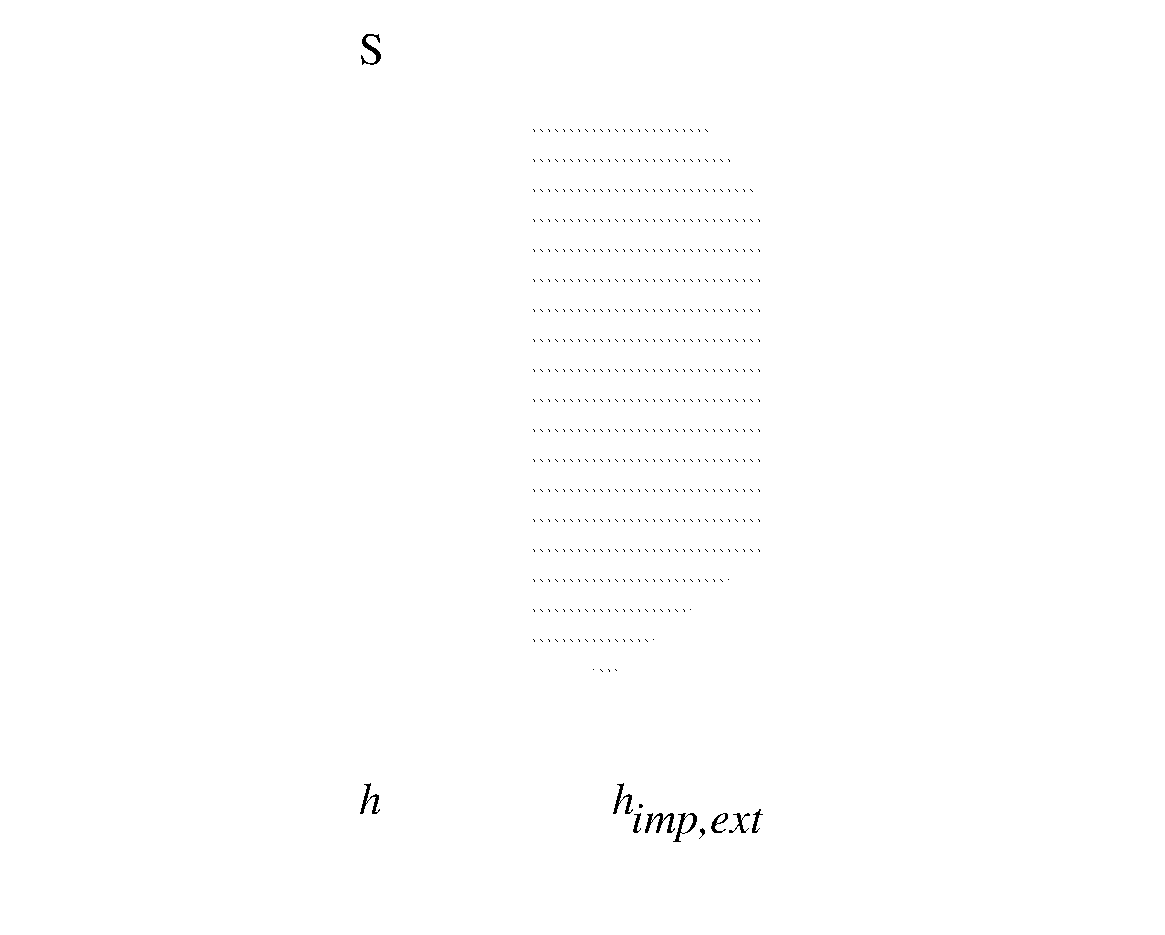
\includegraphics[height=7cm]{\repgraphics/fluxbord}}
\caption{\label{Cfbl_Cfxtcl_fig_flux_cfxtcl}Cellule de bord.}
\end{figure}

\begin{equation}\label{Cfbl_Cfxtcl_eq_flux_cfxtcl}
\begin{array}{l}
    \underbrace{h_{int}(f_{b,int}-f_{I'})}_{\phi_{int}}
  = \underbrace{h_{b}(f_{b,ext}-f_{I'})}_{\phi_{b}}
  = \left\{\begin{array}{ll}
    \underbrace{h_{imp,ext}(f_{imp,ext}-f_{b,ext})}_{\phi_{\text{\it r\'eel
impos\'e}}} &\text{(condition de Dirichlet)}\\
    \underbrace{\phi_{\text{\it imp,ext}}}_{\phi_{\text{\it r\'eel impos\'e}}}
            &\text{(condition de Neumann)}
           \end{array}\right.
\end{array}
\end{equation}


L'\'equation~(\ref{Cfbl_Cfxtcl_eq_fbint_cfxtcl}) rappelle la formulation des
conditions aux limites pour une variable $f$.
\begin{equation}\label{Cfbl_Cfxtcl_eq_fbint_cfxtcl}
f_{b,int}
  = \left\{\begin{array}{cccccl}
    \displaystyle\frac{h_{imp,ext}}{h_{int}+h_r h_{imp,ext} }&f_{imp,ext}&+&
    \displaystyle\frac{h_{int}+h_{imp,ext}(h_r-1)}{h_{int}+h_r h_{imp,ext} }&f_{I'}
                         &\text{(condition de Dirichlet)}\\
    \displaystyle\frac{1}{h_{int}}&\phi_{\text{\it imp,ext}}&+&
    \ &f_{I'}
            &\text{(condition de Neumann)}
           \end{array}\right.
\end{equation}

Les coefficients d'\'echange sont d\'efinis comme suit\footnote{On rappelle que, comme
dans \fort{condli}, $\alpha$ d\'esigne $\lambda+C_p\,\frac{\mu_t}{\sigma_t}$
si $f$ est la temp\'erature,
$\frac{\lambda}{C_p}+\frac{\mu_t}{\sigma_t}$ si $f$ repr\'esente l'enthalpie.
Le coefficient $C$ repr\'esente $C_p$ pour la temp\'erature et vaut
$1$ pour l'enthalpie. La grandeur adimensionnelle $f^+$ est obtenue par
application d'un principe de similitude en paroi~: pour la temp\'erature,
elle d\'epend du nombre de
Prandlt mol\'eculaire, du nombre de Prandtl turbulent et de la distance adimensionnelle \`a la paroi $y^+$ dans la cellule de bord.}~:
\begin{equation}
\left\{\begin{array}{lll}
h_{int}&=&\displaystyle\frac{\alpha}{\overline{I'F}}\\
h_r&=&\displaystyle\frac{h_{int}}{h_{b}} \\
h_b&=&\displaystyle\frac{\phi_b}{f_{b,ext}-f_{I'}}=\frac{\rho\,C\,u_k}{f^+_{I'}}
\end{array}\right.
\end{equation}

Dans \CS, on note les conditions aux limites de mani\`ere g\'en\'erale sous
la forme suivante~:
\begin{equation}
f_{b,int}=A_b + B_b\,f_{I'}
\end{equation}
avec $A_b$ et $B_b$ d\'efinis selon le type des conditions~:
\begin{equation}
\begin{array}{c}
\text{Dirichlet}\left\{\begin{array}{ll}
    A_b = &\displaystyle\frac{h_{imp,ext}}{h_{int}+h_r h_{imp,ext} } f_{imp,ext}\\
    B_b = &\displaystyle\frac{h_{int}+h_{imp,ext}(h_r-1)}{h_{int}+h_r h_{imp,ext} }
                  \end{array}\right.
\text{\ \  Neumann}\left\{\begin{array}{ll}
    A_b = &\displaystyle\frac{1}{h_{int}}\phi_{\text{\it imp,ext}}\\
    B_b = &1
                  \end{array}\right.
\end{array}
\end{equation}

%---------------------------------
\subsubsection{Flux diffusif d'\'energie}
%---------------------------------

Dans le module compressible, on r\'esout une \'equation sur l'\'energie, qui s'\'ecrit, si
l'on excepte tous les termes hormis le flux de diffusion et le terme
instationnaire, pour faciliter la pr\'esentation~:

\begin{equation}
\begin{array}{lll}
\displaystyle\frac{\partial \rho e}{\partial t} &=& - \dive{\,\vect{\Phi}_s}\\
&=& \displaystyle\dive{(K\,\grad{T})} \text{\ \ avec \ \ } K=\lambda+C_p\,\frac{\mu_t}{\sigma_t}\\
&=& \displaystyle\dive{\left(K\,\grad{\frac{e-\frac{1}{2}\,u^2-\varepsilon_{sup}}{C_v}}\right)} \\
&=& \displaystyle\dive{\left(\frac{K}{C_v}\,\grad{(e-\frac{1}{2}\,u^2-\varepsilon_{sup})}\right)} \text{\ \
si \ \ } C_v \text{\ est constant}\\
&=& \displaystyle\dive{\left(\frac{K}{C_v}\,\grad\,e\right)}
-\dive{\left(\frac{K}{C_v}\,\grad{(\frac{1}{2}\,u^2+\varepsilon_{sup})}\right)} \\

\end{array}
\end{equation}

La d\'ecomposition en $e$ et $\frac{1}{2}\,u^2+\varepsilon_{sup}$ est purement
math\'ematique (elle r\'esulte du fait que l'on r\'esout en \'energie alors que
le flux thermique s'exprime en fonction de la temp\'erature). Aussi,  pour imposer un
flux de bord ou une temp\'erature de bord (ce qui revient au m\^eme puisque l'on
impose toujours finalement la conservation du flux normal), on {\it choisit}
de reporter la totalit\'e de la condition \`a la limite sur le terme
$\displaystyle\frac{K}{C_v}\,\grad\,e$
et donc d'annuler le flux associ\'e au terme
$\displaystyle\frac{K}{C_v}\,\grad{(\frac{1}{2}\,u^2+\varepsilon_{sup})}$
(en pratique, pour l'annuler, on se contente de ne pas l'ajouter
au second membre de l'\'equation). Conform\'ement \`a l'approche retenue dans \CS et
rappel\'ee pr\'ec\'edemment, on d\'eterminera donc une valeur de bord {\it
fictive} de l'\'energie qui permette de reconstruire le flux diffusif total
attendu \`a partir
de la discr\'etisation du seul terme $\displaystyle\frac{K}{C_v}\,\grad\,e$.

Remarque : dans la version 1.2.0,
on utilise $\displaystyle
\frac{K}{C_v}=\left(\frac{\lambda}{C_v}+\frac{\mu_t}{\sigma_t}\right)$, \`a
partir de 1.2.1, on utilise la valeur  $\displaystyle
\frac{K}{C_v}=\left(\frac{\lambda}{C_v}+\frac{C_p}{C_v}\frac{\mu_t}{\sigma_t}\right)$.
On notera que le nombre de Prandtl turbulent $\sigma_t$ est associ\'e \`a la variable
r\'esolue et peut \^etre fix\'e par l'utilisateur.


%---------------------------------
\subsubsection{Condition de Neumann}
%---------------------------------

La conservation du flux s'\'ecrit~:

\begin{equation}
    \underbrace{h_{int}(e_{b,int}-e_{I'})}_{\phi_{int}}
    =\underbrace{\phi_{\text{\it imp,ext}}}_{\phi_{\text{\it r\'eel impos\'e}}}
\end{equation}

On a donc dans ce cas~:
\begin{equation}
\left\{\begin{array}{lll}
  A_b &= &\displaystyle\frac{1}{h_{int}}\phi_{\text{\it imp,ext}}\\
  B_b &= &1
\end{array}\right.
\end{equation}


%---------------------------------
\subsubsection{Condition de Dirichlet}
%---------------------------------

On suppose que la condition de Dirichlet porte sur la temp\'erature $T_{b,ext}$.


La conservation du flux s'\'ecrit~:
\begin{equation}\label{Cfbl_Cfxtcl_eq_conservation_flux_cfxtcl}
    \underbrace{h_{int}(e_{b,int}-e_{I'})}_{\phi_{int}\text{\ (forme num\'erique
du flux)}}
  = \underbrace{h_{b}(T_{b,ext}-T_{I'})}_{\phi_{b}\text{ qui int\`egre l'effet
de couche limite}}
  =
    \underbrace{h'_{imp,ext}(T_{imp,ext}-T_{b,ext})}_{\phi_{\text{\it r\'eel
impos\'e}}}
\end{equation}

Avec pour les coefficients d'\'echange~:
\begin{equation}
\left\{\begin{array}{lll}
h_{int}&=&\displaystyle\frac{K}{C_v\,\overline{I'F}}\\
h_b&=&\displaystyle\frac{\phi_b}{T_{b,ext}-T_{I'}}=\frac{\rho\,C_p\,u_k}{T^+_{I'}}
\end{array}\right.
\end{equation}

On tire $T_{b,ext}$
de la seconde partie de l'\'egalit\'e~(\ref{Cfbl_Cfxtcl_eq_conservation_flux_cfxtcl})
traduisant la conservation du flux~:
\begin{equation}
\displaystyle T_{b,ext} = \frac{h'_{imp,ext}\,T_{imp,ext}+h_b\,T_{I'}}{h_b+h'_{imp,ext}}
\end{equation}

En utilisant cette valeur et la premi\`ere partie de l'\'equation de conservation
du flux~(\ref{Cfbl_Cfxtcl_eq_conservation_flux_cfxtcl}), on obtient~:
\begin{equation}
e_{b,int} = \frac{h_b\,h'_{imp,ext}}{h_{int}\,(h_b+h'_{imp,ext})}\,(T_{imp,ext}-T_{I'})+e_{I'}
\end{equation}

On utilise alors
$\displaystyle T_{I'}=\frac{1}{C_v}\left(e_{I'}-\frac{1}{2}u^2_{i}-\varepsilon_{sup,i}\right)$ pour
\'ecrire (sans reconstruction pour la vitesse et $\varepsilon_{sup}$)~:
\begin{equation}
\displaystyle e_{b,int} =
\frac{ -\frac{h_b\,h'_{imp,ext}}{C_v}+h_{int}\,(h_b+h'_{imp,ext}) }
     { h_{int}\,(h_b+h'_{imp,ext}) } \,e_{I'}
+\frac{h_b\,h'_{imp,ext}}{h_{int}\,(h_b+h'_{imp,ext})}\,
  \left(T_{imp,ext}+\frac{\frac{1}{2}u^2_{i}+\varepsilon_{sup,i}}{C_v}\right)
\end{equation}


Et on a donc, avec $\displaystyle h'_r=\frac{h_{int}}{\frac{h_b}{C_v}}$~:
\begin{equation}
\displaystyle e_{b,int} =
\underbrace{\frac{ h'_{imp,ext} }{ C_v\,h_{int}+h'_r\,h'_{imp,ext} }\,
  \left(C_v\,T_{imp,ext}+\frac{1}{2}u^2_{i}+\varepsilon_{sup,i}\right)}_{A_b}
+\underbrace{\frac{ C_v\,h_{int}+h'_{imp,ext}(h'_r-1) }{ C_v\,h_{int}+h'_r\,h'_{imp,ext} }}_{B_b}\,e_{I'}
\end{equation}

Avec ces notations, $h_b$ est le coefficient habituellement calcul\'e pour la
temp\'erature.

Le coefficient $h'_{imp,ext}$ est le coefficient d'\'echange externe qui est
impos\'e pour la temp\'erature\footnote{Le coefficient $h'_{imp,ext}$
est utile pour les cas o\`u l'on
souhaite relaxer la condition \`a la limite~:
pour la temp\'erature, cela correspond \`a imposer une valeur sur la face
externe d'une paroi unidimensionnelle id\'eale, sans inertie,
caract\'eris\'ee par un simple coefficient d'\'echange.}.
Pour obtenir l'\'equivalent dimensionnel de $h'_{imp,ext}$ pour l'\'energie,
il faut diviser sa valeur par $C_v$ (ce qui ne fait pas de diff\'erence dans
la majorit\'e des cas, car il est habituellement pris infini).

%%%%%%%%%%%%%%%%%%%%%%%%%%%%%%%%%%
%%%%%%%%%%%%%%%%%%%%%%%%%%%%%%%%%%
\section{Mise en \oe uvre}
%%%%%%%%%%%%%%%%%%%%%%%%%%%%%%%%%%
%%%%%%%%%%%%%%%%%%%%%%%%%%%%%%%%%%

%=================================
\subsection{Introduction}
%=================================

Les conditions aux limites sont impos\'ees par une suite de sous-programmes,
dans la mesure o\`u l'on a cherch\'e \`a rester coh\'erent avec la structure
standard de \CS.

Dans \fort{ppprcl} (appel\'e par \fort{precli}), on initialise les tableaux
avant le calcul des conditions aux limites~:
\begin{itemize}
\item \var{IZFPPP} (num\'ero de zone, inutilis\'e, fix\'e \`a z\'ero),
\item \var{IA(IIFBRU)} (rep\'erage des faces de bord pour
lesquelles on applique un sch\'ema de Rusanov~: initialis\'e \`a z\'ero,
on imposera la valeur 1 dans \fort{cfrusb} pour les faces auxquelles on applique le sch\'ema
de Rusanov)
\item \var{IA(IIFBET)} (rep\'erage des faces de paroi \`a temp\'erature ou
\`a flux thermique impos\'e~: initialis\'e \`a 0, on imposera la valeur 1
dans \fort{cfxtcl} lorsque la temp�rature ou le flux est impos�),
\item \var{RCODCL(*,*,1)} (initialis\'e \`a \var{-RINFIN} en pr\'evision
du traitement des sorties r\'eentrantes pour lesquelles l'utilisateur
aurait fourni une valeur \`a imposer en Dirichlet),
\item flux convectifs de bord pour la quantit\'e de mouvement et l'\'energie
(initialis\'es \`a z\'ero).
\end{itemize}


\bigskip
Les types de fronti\`ere (\var{ITYPFB}) et les valeurs n\'ecessaires
(\var{ICODCL}, \var{RCODCL}) sont impos\'es par l'utilisateur dans \fort{uscfcl}.

On convertit ensuite ces donn\'ees dans \fort{condli} pour qu'elles
soient directement utilisables lors du calcul des matrices et des seconds membres.

Pour cela, \fort{cfxtcl} permet de r\'ealiser le calcul des valeurs de bord et,
pour certaines fronti\`eres, des flux convectifs. On fait appel,
en particulier,
\`a \fort{uscfth} (utilisation de la thermodynamique) et \`a \fort{cfrusb}
(flux convectifs par le sch\'ema de Rusanov). Lors de ces calculs, on utilise
\var{COEFA} et \var{COEFB} comme tableaux de travail (transmission de valeurs
\`a \fort{uscfth} en particulier) afin de renseigner \var{ICODCL} et
\var{RCODCL}.
Apr\`es \fort{cfxtcl},
le sous-programme \fort{typecl} compl\`ete quelques valeurs par d\'efaut
de \var{ICODCL} et de \var{RCODCL}, en particulier pour les scalaires passifs.

Apr\`es \fort{cfxtcl} et \fort{typecl}, les tableaux \var{ICODCL} et \var{RCODCL}
sont complets. Ils sont utilis\'es dans la suite de \fort{condli} et en particulier
dans \fort{clptur} pour construire les tableaux \var{COEFA} et \var{COEFB}
(pour l'\'energie, on dispose de deux couples (\var{COEFA}, \var{COEFB}) afin de
traiter les parois).

On pr\'esente ci-apr\`es les points dont l'implantation diff\`ere
de l'approche standard. Il s'agit de
l'utilisation d'un sch\'ema de Rusanov pour le calcul des flux convectifs
en entr\'ee et sortie (hormis sortie supersonique)
et du mode de calcul des flux diffusifs d'\'energie en paroi.
On insiste en particulier sur l'impact des conditions aux limites
sur la construction des seconds membres de l'\'equation de la quantit\'e
de mouvement et de l'\'equation de l'\'energie (\fort{cfqdmv} et \fort{cfener}).

%=================================
\subsection{Flux de Rusanov pour le calcul des flux convectifs en entr\'ee et sortie}
%=================================

Le sch\'ema de Rusanov est utilis\'e pour calculer des flux convectifs de bord
(masse, quantit\'e de mouvement et \'energie) aux entr\'ees et des sorties
de type IESICF, ISOPCF, IERUCF, IEQHCF.

La gestion des conditions aux limites est diff\'erente de celle adopt\'ee
classiquement dans \CS, bien que l'on se soit efforc\'e de s'y conformer le
mieux possible.

En volumes finis, il faut disposer de conditions aux
limites pour trois utilisations principales au moins~:
         \begin{itemize}
        \item imposer les flux de convection,
        \item imposer les flux de diffusion,
        \item calculer les gradients pour les reconstructions.
        \end{itemize}
Dans l'approche standard de \CS, les conditions aux limites sont d\'efinies par
variable et non pas par terme discret\footnote{Par exemple, pour un scalaire
convect\'e et diffus\'e, on d\'efinit une valeur de bord unique {\it pour le scalaire}
et non pas une valeur de bord pour le {\it flux convectif} et une valeur de bord
pour le {\it flux diffusif}.}. On dispose donc, {\it pour chaque variable},
d'une valeur de bord dont devront \^etre d\'eduits les flux de
convection, les flux de diffusion et les gradients\footnote{N\'eanmoins, pour
certaines variables comme la vitesse par exemple, \CS dispose de deux valeurs
de bord (et non pas d'une seule) afin de pouvoir imposer de mani\`ere
ind\'ependante le gradient normal et le flux de diffusion.}.
Ici, avec l'utilisation d'un sch\'ema de
Rusanov, dans lequel le flux convectif est trait\'e dans son ensemble,
il est imp\'eratif
de disposer d'un moyen d'imposer directement sa valeur au bord\footnote{Il
serait possible de calculer une valeur de bord fictive des variables d'\'etat qui
permette de retrouver le flux convectif calcul\'e par le sch\'ema de Rusanov,
mais cette valeur ne permettrait pas d'obtenir
un flux de diffusion et un gradient satisfaisants.}.

Le flux convectif calcul\'e par le sch\'ema de Rusanov
sera ajout\'e directement au second membre
des \'equations de masse, de quantit\'e de mouvement et d'\'energie. Comme ce
flux contient, outre la contribution des termes convectifs ``usuels''
($\dive(\vect{Q})$, $\dive(\vect{u}\otimes\vect{Q})$ et
$\dive(\vect{Q}\,e)$), celle des termes en $\grad\,P$ (quantit\'e de
mouvement) et $\dive(\vect{Q}\,\frac{P}{\rho})$
(\'energie), il faut veiller \`a ne pas
ajouter une seconde fois les termes de bord issus de  $\grad\,P$ et de
$\dive(\vect{Q}\,\frac{P}{\rho})$
au second membre des \'equations de quantit\'e de
mouvement et d'\'energie.


Pour la masse, le flux convectif calcul\'e par le sch\'ema de Rusanov
d\'efinit simplement le flux de masse au bord
(\var{PROPFB(IFAC,IPPROB(IFLUMA(ISCA(IENERG(IPHAS)))))}).

Pour la quantit\'e de mouvement, le flux convectif calcul\'e par le sch\'ema de
Rusanov  est stock\'e dans les tableaux
\var{PROPFB(IFAC,IPPROB(IFBRHU(IPHAS)))}, \var{PROPFB(IFAC,IPPROB(IFBRHV(IPHAS)))} et
\var{PROPFB(IFAC,IPPROB(IFBRHW(IPHAS)))}. Il est ensuite ajout\'e au second membre de
l'\'equation directement dans \fort{cfqdmv} (boucle sur les faces de bord).
Comme ce flux contient la contribution du terme convectif usuel
$\divv(\vect{u}\otimes\vect{Q})$, il ne faut pas l'ajouter dans
le sous-programme \fort{cfbsc2}.
De plus, le flux convectif calcul\'e par le sch\'ema de Rusanov
contient la contribution du
gradient de pression. Or, le gradient de pression est calcul\'e dans
\fort{cfqdmv} au moyen de \fort{grdcel} et ajout\'e au second membre
sous forme de contribution volumique (par cellule)~: il faut donc retirer
la contribution des faces de bord auxquelles est appliqu\'e le sch\'ema de
Rusanov, pour ne pas la compter deux fois (cette op\'eration est r\'ealis\'ee
dans \fort{cfqdmv}).

Pour l'\'energie, le flux convectif calcul\'e par le sch\'ema de
Rusanov est stock\'e dans le tableau
\var{PROPFB(IFAC,IPPROB(IFBENE(IPHAS)))}. Pour les faces auxquelles n'est pas
appliqu\'e le sch\'ema de Rusanov, on ajoute la contribution
du terme de transport de pression $\dive(\vect{Q}\,\frac{P}{\rho})$
au second membre de l'\'equation dans \fort{cfener}
et on compl\`ete le second membre dans \fort{cfbsc2} avec la contribution du
terme convectif usuel $\dive(\vect{Q}\,e)$. Pour les faces auxquelles est
appliqu\'e le sch\'ema de Rusanov, on ajoute directement le flux de Rusanov au second
membre de l'\'equation dans \fort{cfener}, en lieu et place de la contribution
du terme de transport de pression et l'on prend garde de ne pas
comptabiliser une seconde fois le flux convectif usuel
$\divv(\vect{Q}\,e)$ dans le sous-programme \fort{cfbsc2}.

C'est l'indicateur \var{IA(IIFBRU)}
(renseign\'e dans \fort{cfrusb}) qui permet, dans \fort{cfbsc2},
\fort{cfqdmv} et \fort{cfener},
de rep\'erer les faces de bord pour lesquelles on a calcul\'e
un flux convectif avec le sch\'ema de Rusanov.


%=================================
\subsection{Flux diffusif d'\'energie}
%=================================

%---------------------------------
\subsubsection{Introduction}
%---------------------------------

Une condition doit \^etre fournie sur toutes les fronti\`eres pour le calcul du
flux diffusif d'\'energie.

Il n'y a pas lieu de
s'\'etendre particuli\`erement sur le traitement de certaines fronti\`eres.
Ainsi, aux entr\'ees et sorties, on dispose
d'une valeur de bord (issue de la r\'esolution du probl\`eme
de Riemann)
que l'on utilise dans la formule discr\`ete classique donnant le
flux\footnote{Les valeurs de $u^2$ et de $\varepsilon_{sup}$ ne sont pas
reconstruites pour le calcul du gradient au bord dans
$\displaystyle\dive{\left(\frac{K}{C_v}\,\grad{(\frac{1}{2}\,u^2+\varepsilon_{sup})}\right)}$}.
La situation est simple aux sym\'etries \'egalement, o\`u un flux nul est impos\'e.

Par contre, en paroi, les conditions de temp\'erature ou de flux thermique
impos\'e doivent \^etre trait\'ees avec plus d'attention, en particulier
lorsqu'une couche limite turbulente est pr\'esente.

%---------------------------------
\subsubsection{Coexistence de deux conditions de bord}
%---------------------------------

Comme indiqu\'e dans la partie "discr\'etisation",
les conditions de temp\'erature ou de flux conductif
impos\'e en paroi se traduisent,
pour le flux d'\'energie, au travers du terme
$\displaystyle\dive{\left(\frac{K}{C_v}\,\grad\,e\right)}$,
en imposant une condition de flux nul sur le terme
$\displaystyle-\dive{\left(\frac{K}{C_v}\,\grad{(\frac{1}{2}\,u^2+\varepsilon_{sup})}\right)}$.
Les faces IFAC
concern\'ees sont rep\'er\'ees dans \fort{cfxtcl} par l'indicateur
\var{IA(IIFBET+IFAC-1+(IPHAS-1)*NFABOR) = 1} (qui vaut 0 sinon, initialis\'e
dans \fort{ppprcl}).

Sur ces faces,
on calcule une valeur de bord de l'\'energie, qui, introduite dans la
formule g\'en\'erale de flux utilis\'ee au bord dans \CS, permettra de retouver le
flux souhait\'e. La valeur de bord est une simple valeur num\'erique sans
signification physique et ne doit \^etre utilis\'ee que pour calculer le flux
diffusif.

En plus de cette valeur de bord destin\'ee \`a retrouver le
flux diffusif, il est n\'ecessaire de disposer
d'une seconde valeur de bord de l'\'energie afin de pouvoir en calculer le
gradient.

Ainsi, comme pour la vitesse en $k-\varepsilon$, il est n\'ecessaire de
disposer pour l'\'energie de deux couples de coefficients
(\var{COEFA},\var{COEFB}), correspondant \`a deux valeurs de bord distinctes,
dont l'une est utilis\'ee pour le calcul du flux diffusif sp\'ecifiquement.

%---------------------------------
\subsubsection{Calcul des \var{COEFA} et \var{COEFB} pour les faces de paroi
\`a temp\'erature impos\'ee}
%---------------------------------

Les  faces de paroi  \var{IFAC} \`a temp�rature impos\'ee sont identif\'ees par
l'utilisateur dans \fort{uscfcl} au moyen de  l'indicateur
\var{ICODCL(IFAC,ISCA(ITEMPK(IPHAS)))=5} (noter que
ce tableau est associ\'e \`a la temp\'erature).

Dans \fort{cfxtcl}, on impose alors \var{ICODCL(IFAC,ISCA(IENERG(IPHAS)))=5} et
on calcule la quantit\'e
$C_v\,T_{imp,ext}+\frac{1}{2}u^2_{I}+\varepsilon_{sup,I}$, que l'on
stocke dans \var{RCODCL(IFAC,ISCA(IENERG(IPHAS)),1)} (on ne reconstruit pas les
valeurs de $u^2$ et $\varepsilon_{sup}$ au bord, cf. \S\ref{Cfbl_Cfxtcl_prg_a_traiter}).

\`A partir de ces valeurs de \var{ICODCL} et \var{RCODCL},
on renseigne ensuite dans \fort{clptur}
les tableaux de conditions aux limites  permettant le calcul du flux~:
\var{COEFA(*,ICLRTP(ISCA(IENERG(IPHAS)),ICOEFF))} et
\var{COEFB(*,ICLRTP(ISCA(IENERG(IPHAS)),ICOEFF))} (noter
l'indicateur \var{ICOEFF} qui renvoie aux coefficients d\'edi\'es au flux
diffusif).


%---------------------------------
\subsubsection{Calcul des \var{COEFA} et \var{COEFB} pour les faces de paroi
\`a flux thermique impos\'e}
%---------------------------------

Les  faces de paroi  \var{IFAC} \`a flux thermique
impos\'e sont identif\'ees par
l'utilisateur dans \fort{uscfcl} au moyen de  l'indicateur
\var{ICODCL(IFAC,ISCA(ITEMPK(IPHAS)))=3} (noter que le tableau est
associ\'e \`a la temp\'erature).

Dans \fort{cfxtcl}, on impose alors \var{ICODCL(IFAC,ISCA(IENERG(IPHAS)))=3} et
on transf\`ere la valeur du flux de  \var{RCODCL(IFAC,ISCA(ITEMPK(IPHAS)),3)}
\`a \var{RCODCL(IFAC,ISCA(IENERG(IPHAS)),3)}.

\`A partir de ces valeurs de \var{ICODCL} et \var{RCODCL},
on renseigne ensuite dans \fort{condli} les tableaux de conditions aux limites
permettant le calcul du flux,
\var{COEFA(*,ICLRTP(ISCA(IENERG(IPHAS)),ICOEFF))} et
\var{COEFB(*,ICLRTP(ISCA(IENERG(IPHAS)),ICOEFF))} (noter
l'indicateur \var{ICOEFF} qui renvoie aux coefficients d\'edi\'es au flux
diffusif).

%---------------------------------
\subsubsection{Gradient de l'\'energie en paroi \`a temp\'erature ou \`a flux thermique impos\'e}
%---------------------------------

Dans les deux cas (paroi \`a temp\'erature ou \`a flux thermique impos\'e),
on utilise les tableaux
\var{COEFA(*,ICLRTP(ISCA(II),ICOEF))},
\var{COEFB(*,ICLRTP(ISCA(II),ICOEF))} (noter le \var{ICOEF}) pour disposer d'une
condition de flux nul pour l'\'energie (avec \var{II=IENERG(IPHAS)}) et
pour la temp\'erature (avec \var{II=ITEMPK(IPHAS)})
si un calcul de gradient est requis.

Un gradient est en particulier utile pour les reconstructions
de l'\'energie sur maillage non orthogonal.
Pour la temp\'erature, il s'agit d'une pr\'ecaution, au cas
o\`u l'utilisateur aurait besoin d'en calculer le gradient.

%---------------------------------
\subsubsection{Autres fronti\`eres que les parois \`a temp\'erature ou \`a flux thermique impos\'e}
%---------------------------------

Pour les fronti\`eres qui ne sont pas des parois \`a temp\'erature ou
\`a flux thermique impos\'e, les conditions aux limites de l'\'energie et
de la temp\'erature sont compl\'et\'ees classiquement dans \fort{condli} selon
les choix faits dans \fort{cfxtcl} pour \var{ICODCL} et \var{RCODCL}.

En particulier,
dans le cas de conditions de Dirichlet sur l'\'energie (entr\'ees, sorties), les
deux jeux de conditions aux limites sont identiques (tableaux
\var{COEFA}, \var{COEFB} avec \var{ICOEFF} et \var{ICOEF}).

Si un flux est impos\'e pour l'\'energie totale (condition assez rare,
l'utilisateur ne raisonnant pas,
d'ordinaire, en \'energie totale), on le stocke au moyen de
\var{COEFA(*,ICLRTP(ISCA(IENERG(IPHAS)),ICOEFF))} et
\var{COEFB(*,ICLRTP(ISCA(IENERG(IPHAS)),ICOEFF))} (tableaux associ\'es au flux
diffusif). Pour le gradient, une condition de flux nul est stock\'ee
dans
\var{COEFA(*,ICLRTP(ISCA(IENERG(IPHAS)),ICOEF))} et
\var{COEFB(*,ICLRTP(ISCA(IENERG(IPHAS)),ICOEF))}. On peut remarquer que les deux
jeux de conditions aux limites sont identiques pour les faces de sym\'etrie.

%---------------------------------
\subsubsection{Impact dans \fort{cfener}}
%---------------------------------

Lors de la construction des seconds membres, dans \fort{cfener}, on utilise les
conditions aux limites stock\'ees dans les tableaux associ\'es au flux
diffusif
\var{COEFA(*,ICLRTP(ISCA(IENERG(IPHAS)),ICOEFF))} et
\var{COEFB(*,ICLRTP(ISCA(IENERG(IPHAS)),ICOEFF))} pour le terme de flux diffusif
$\displaystyle\dive{\left(\frac{K}{C_v}\,\grad\,e\right)}$
en prenant soin d'annuler la contribution de bord du terme
$\displaystyle-\dive{\left(\frac{K}{C_v}\,\grad{(\frac{1}{2}\,u^2+\varepsilon_{sup})}\right)}$
sur les faces pour lesquelles cette condition
prend les deux termes en compte, c'est-\`a-dire sur les faces pour lesquelles
\var{IA(IIFBET+IFAC-1+(IPHAS-1)*NFABOR) = 1}.

Pour tous les autres termes qui requi\`erent une valeur de bord, on utilise les
conditions aux limites que l'on a stock\'ees au moyen des deux tableaux
\var{COEFA(*,ICLRTP(ISCA(IENERG(IPHAS)),ICOEF))} et
\var{COEFB(*,ICLRTP(ISCA(IENERG(IPHAS)),ICOEF))}. Ces conditions sont
donc en particulier utilis\'ees pour le calcul du gradient de l'\'energie,
lors des reconstructions sur maillage non orthogonal.


\newpage
%%%%%%%%%%%%%%%%%%%%%%%%%%%%%%%%%%
%%%%%%%%%%%%%%%%%%%%%%%%%%%%%%%%%%
\section{Points \`a traiter}
%%%%%%%%%%%%%%%%%%%%%%%%%%%%%%%%%%
%%%%%%%%%%%%%%%%%%%%%%%%%%%%%%%%%%
\label{Cfbl_Cfxtcl_prg_a_traiter}%
% propose en patch 1.2.1
%Corriger \fort{ppprcl} pour que l'indicateur
%\var{IA(IIFBET+IFAC-1+(IPHAS-1)*NFABOR)} soit
%initialis\'e \`a 0, positionn\'e \`a 1 aux faces de paroi \`a temp\'erature
%ou flux thermique impos\'e. Dans \fort{cfener}, lorsque l'indicateur vaudra 1,
%on ne prendra pas en compte le flux correspondant \`a
%$\displaystyle-\dive{\left(\frac{K}{C_v}\,\grad{(\frac{1}{2}\,u^2+\varepsilon_{sup})}\right)}$.

% propose en patch 1.2.1
%Pour l'\'energie, on utilise comme diffusivit\'e turbulente la valeur
%$\displaystyle \frac{K}{C_v}=\frac{\lambda}{C_v}+\frac{\mu_t}{\sigma_t}$.
%Par coh\'erence avec une \'equation
%portant sur la temp\'erature, il serait plus logique d'utiliser
%$\displaystyle \frac{K}{C_v}=\frac{\lambda}{C_v}+\frac{C_p}{C_v}\,\frac{\mu_t}{\sigma_t}$.
%On peut temporairement utiliser le nombre de Prandtl turbulent pour prendre en compte
%le rapport $\displaystyle\frac{C_p}{C_v}$, mais il serait
%souhaitable de corriger en ce sens le calcul de \var{W1} pour \fort{viscfa} dans
%le sous-programme \fort{cfener} et le calcul similaire de \var{HINT} dans
%\fort{condli} et \fort{clptur} (RAS pour les conversions en couplage avec \syrthes).

Apporter un compl\'ement de test sur une cavit\'e ferm\'ee
sans vitesse et sans gravit\'e, avec flux de bord ou temp\'erature de bord impos\'ee.
Il semble que le transfert d'\'energie {\it via} les termes de pression g\'en\`ere de
fortes vitesses non physiques dans la premi\`ere maille de paroi et que la
conduction thermique ne parvienne pas \`a \'etablir le profil de temp\'erature
recherch\'e. Il est \'egalement possible que la condition de bord sur la pression
g\'en\`ere une perturbation (une extrapolation pourrait se r\'ev\'eler
indispensable).

Il pourrait \^etre utile de g\'en\'eraliser \`a l'incompressible l'approche
utilis\'ee en compressible pour unifier simplement le traitement
des sorties de type 9 et 10.

Il pourrait \^etre utile d'\'etudier plus en d\'etail l'influence de la non
orthogonalit\'e des mailles en sortie supersonique (pas de reconstruction,
ce qui n'est pas consistant pour les flux de diffusion).

De m\^eme, il serait utile d'\'etudier l'influence de l'absence de
reconstruction pour la vitesse et $\varepsilon_{sup}$ dans la relation
$\displaystyle T_{I'}=\frac{1}{C_v}\left(e_{I'}-\frac{1}{2}u^2_{i}-\varepsilon_{sup,i}\right)$
utilis\'ee pour les parois \`a temp\'erature impos\'ee.

Apporter un compl\'ement de documentation pour le couplage avec \syrthes (conversion
\'energie temp\'erature). Ce n'est pas une priorit\'e.

Pour les thermodynamiques \`a $\gamma$ variable, il sera n\'ecessaire de
modifier non
seulement \fort{uscfth} mais \'egalement \fort{cfrusb} qui doit disposer de
$\gamma$ en argument.

Pour les thermodynamiques \`a $C_v$ variable, il sera n\'ecessaire de
prendre en compte un terme en $\grad\,C_v$, issu des flux diffusifs,
au second membre de l'\'equation de
l'\'energie (on pourra cependant remarquer qu'actuellement, en incompressible,
on n\'eglige le terme en $\grad\,C_p$ dans l'\'equation de l'enthalpie).
